\newpage
\begin{problem}
Шесть определений непрерывной функции.
\end{problem}

$$\varnothing$$

\newpage
\begin{problem}
Определение непрерывности в точке справа и слева. Критерий непрерывности в терминах непрерывности слева и справа (Предложение 1, Лекция 13).
\end{problem}

$$\varnothing$$

\newpage
\begin{problem}
Локальные свойства непрерывных функций.
\end{problem}

$$\varnothing$$

\newpage
\begin{problem}
Теорема о композиции непрерывных функций. Точка разрыва.
\end{problem}

$$\varnothing$$

\newpage
\begin{problem}
Устранимый разрыв, разрыв первого рода и разрыв второго рода. Разрывы монотонной
на интервале функции. Определение непрерывной на множестве функции.
\end{problem}

$$\varnothing$$

\newpage
\begin{problem}
Теорема о нуле непрерывной на отрезке функции (Теорема 1, Лекция 13). Определение
ограниченной на множестве функции. 1-я теорема Вейерштрасса.
\end{problem}

$$\varnothing$$

\newpage
\begin{problem}
2-я теорема Вейерштрасса Теорема Больцано – Коши о промежуточном значении.
\end{problem}

$$\varnothing$$

\newpage
\begin{problem}
Определение равномерной непрерывности. Теорема Гейне – Кантора.
\end{problem}

\begin{definition}
    Функция $f,$ определенная на множестве $E,$
    называется равномерно непрерывной на этом множестве,
    если для любого числа $\varepsilon>0$ существует
    такое $\delta>0,$ что при всех таких
    $x_1, x_2\in E,$ что $|x_1-x_2|<\delta,$ выполнено
    неравенство
    $$
        |f(x_1)-f(x_2)|<\varepsilon.
    $$
\end{definition}

\begin{theorem}(\textbf{Гейне -- Кантора о равномерной
        непрерывности}).
    Функция $f,$ непрерывная на отрезке $[a, b],$
    равномерно непрерывна на этом отрезке.
\end{theorem}

\newpage
\begin{problem}
Обратная функция. Критерий непрерывности монотонной функции. Теорема об обратной функции.
\end{problem}

\begin{definition}
    Пусть функция $f:E\to D$
    осуществляет биекцию между $E$ и $D.$
    Если каждому $y \in D$ поставить в соответствие
    то $x \in E,$ для которого $f(x)=y,$ то тем
    самым будет определена функция, отображающая
    множество $D$ во множество $E.$ Она называется
    \textbf{обратной} для функции $f$ и обозначается
    $f^{-1}.$ Таким образом, $f^{-1}: D\rightarrow E.$
\end{definition}
\begin{theorem}(\textbf{Критерий непрерывности монотонной
        функции}).
    Монотонная на отрезке $[a, b]$ функция $f,$ непрерывна
    на  этом отрезке тогда и только тогда,
    когда множеством её значений является отрезок
    с концами $f(a)$ и $f(b)$.
\end{theorem}
\begin{theorem}(\textbf{Теорема об обратной
        функции.})
    Пусть функция $f$ непрерывна и строго монотонна
    (то есть возрастает или
    убывает) на отрезке $[a, b].$ Тогда функция $f$
    имеет обратную функцию $f^{-1}$, определенную
    на отрезке с концами $f(a)$ и $f(b),$ причём
    $f^{-1}$ строго монотонна и непрерывна на отрезке
    с концами $f(a)$ и $f(b)$ и характер
    монотонности функций $f$ и $f^{-1}$
    одинаковый.
\end{theorem}
\newpage
\begin{problem}
Определение дифференцируемой функции. Определение дифференциала. Дифференциал как линейная функция (Лекция 16).
\end{problem}

\begin{definition}
    Функция $f,$ определённая в некоторой окрестности
    точки $a,$ называется \textbf{дифференцируемой}
    в точке $a,$ если существуют такие число $A$
    и функция $\alpha,$ что при всех $h$ из некоторой
    проколотой окрестности нуля выполнено равенство
    $$
        f(a+h)-f(a)=Ah+\alpha(h)h, \eqno(1)
    $$
    где $\lim\limits_{h\rightarrow0}\alpha(h)=0.$
    При этом $A$ и $\alpha$ зависят и от точки
    $a,$ поэтому часто равенство (1) записывают
    в виде
    $$
        f(a+h)-f(a)=A(a)h+\alpha(a, h)h.
    $$
\end{definition}
\begin{definition}
    Функция $h\mapsto Ah$ называется \textbf{дифференциалом}
    функции $f$ в точке $a.$ Она обозначается $df(a)$ или
    $df|_{x=a},$ то есть
    $df(a)(h)=df(h)|_{x=a}=Ah.$
\end{definition}

Ещё раз подчеркнём, что
равенство записано в фиксированной точке
$a,$ то есть оно зависит от точки $a.$ Другими словами,
число $A,$ вообще говоря, разное при разных $a.$

Здесь символ $df(a)$ нужно воспринимать как обозначение
функции, то есть как \emph{цельный} символ.

Отметим два очевидных наблюдения для функции $h\mapsto Ah:$
во-первых
$$\forall \lambda\in\R \
    df(a)(\lambda h)=A\lambda h=
    \lambda Ah,
$$
а во-вторых
$$df(a)(h_1+h_2)=A(h_1+h_2)=Ah_1+Ah_2.
$$
Так как здесь $A$ -- число, то свойства очевидны.
Однако позже мы увидим, что дифференциал функции
многих переменных также обладает аналогичными свойствами.
Выполнение этих свойств по определению
означает, что \emph{дифференциал
    является линейной функцией от $h.$}

\newpage
\begin{problem}
Определение производной. Связь дифференцируемости и производной (Предложение
1, Лекция 16). Определение касательной.
\end{problem}

\begin{definition}
    Если существует предел
    $\lim\limits_{h\rightarrow0}\frac{f(a+h)-f(a)}{h},$
    то он называется производной функции $f$ в точке
    $a.$ Другая форма записи предела:
    $\lim\limits_{x\rightarrow a}\frac{f(x)-f(a)}{x-a}.$
    Производная функции $f$ в точке $a$ обозначается
    символом $f'(a)$ или $\frac{df}{dx}(a)$
    (второе обозначение позже обсудим подробно).
\end{definition}

\begin{proposition}
    Функция $f$ дифференцируема в точке $a$
    тогда и только тогда, когда в точке
    $a$ существует производная этой функции $f'(a).$
    При этом $df(h)|_{x=a}=f'(a)h.$
\end{proposition}

Изучим
\emph{геометрическую интерпретацию производной
    и дифференциала}.
Из равенства $h=x-a$ получим, что дифференцируемая
функция может быть записана в виде $f(x)=f(a)+
    f'(a)(x-a)+\alpha(x)(x-a),$ где $\lim\limits_{
        x\rightarrow a}\alpha(x)=0.$ Это значит, что в
некоторой окрестности точки $a$ функция $f$
приближается функцией $x\mapsto f(a)+f'(a)(x-a).$
Таким образом, локально (то есть в некоторой
окрестности точки $a$) график функции $f$
выглядит "почти" как прямая. Сама прямая
$y=f'(a)(x-a)+f(a)$ называется
\emph{касательной} к графику функции $f$ в точке
$a.$ Производная $f'(a)$
является тангенсом угла наклона касательной
к положительному направлению оси $Ox.$
На рисунке 1 красным цветом изображена
касательная. \begin{figure}[h!]
    \center{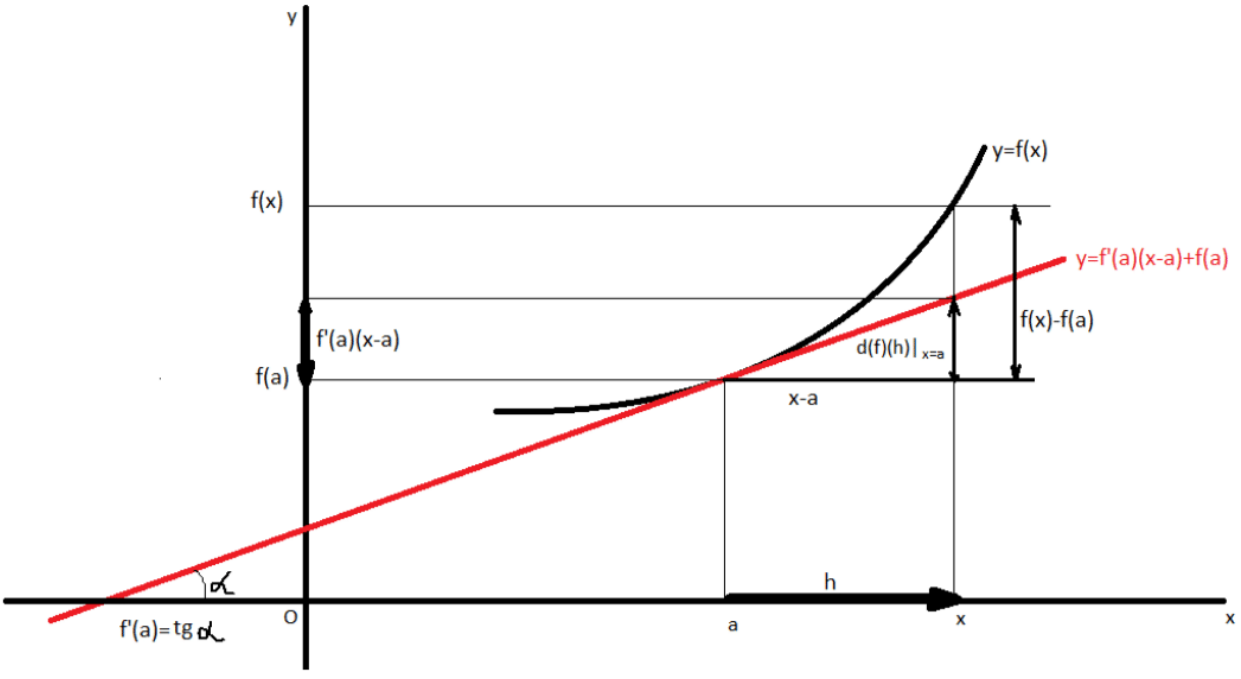
\includegraphics[scale=0.45]{Касательная.png}}
    \caption{Функция "сливается" с касательной.}
    \label{fig:image}
\end{figure} Обратим внимание, что
график функции и касательной неразличимы
в некоторой окрестности.
Приведём несколько примеров на вычисление
производных с помощью определения производной.

\newpage
\begin{problem}
Непрерывность дифференцируемой функции. Определение равномерной сходимости.
\end{problem}

\begin{proposition}
    Пусть функция $f$ дифференцируема
    в точке $a.$ Тогда $f$ непрерывна в точке $a.$
\end{proposition}
\begin{definition}
Функциональная последовательность
$\{f_n(x)\}_{n = 1}^\infty$
\textbf{сходится равномерно} к функции $f(x)$
на множестве $X$, если
$$\forall \varepsilon > 0 \ \exists N
\in \mathbb N: \ \forall n > N \ \forall x \in X
\ |f_n(x) - f(x)| < \varepsilon.
$$
Обозначение: $f_n(x) \underset{X}\rightrightarrows f(x).$
\end{definition}

\newpage
\begin{problem}
Формулировка теоремы о равномерной сходимости последовательности непрерывных
функций. Пример Вейерштрасса непрерывной, но недифференцируемой функции.
\end{problem}
\begin{theorem} (\textbf{Непрерывность предела
равномерно сходящейся последовательности}).
Пусть $X$ -- область сходимости
функциональной последовательности
$\{f_n\}.$
Пусть $\forall n \in \N \ f_n(x) \in C(x_0), \ x_0\in X.$
Пусть $f_n(x) \underset{X}\rightrightarrows f(x).$
Тогда $f(x) \in C(x_0).$
\end{theorem}
С помощью теоремы о непрерывности предела равномерно
сходящейся последовательности можно построить пример
функции, которая в каждой точке непрерывна,
но ни в одной точке не является дифференцируемой.
Для этого рассмотрим следующую последовательность
функций:
\begin{multline*}
f_0(x) = \sin x, \ f_1(x) = \sin x + \frac{1}{2} \sin 8x,
\ f_2(x) = \sin x + \frac{1}{2} \sin 8x +
\frac{1}{4} \sin 64x, \ ...,\\
f_n(x) = \sum\limits_{k=0}\limits^{n}\frac{1}{2^k} \sin 8^k x.
\end{multline*}
Покажем, что эта последовательность функций имеет предел
при каждом $x\in\R,$ то есть областью сходимости
является вся вещественная прямая.
Действительно, при фиксированном $x$
$$
\sum\limits_{k=0}\limits^{n}\left|\frac{1}{2^k}
\sin 8^k x\right|\leq
\sum\limits_{k=0}\limits^{n}\frac{1}{2^k}\leq2,
$$
то есть частичные суммы ряда
$\sum\limits_{k=0}\limits^{+\infty}
\left|\frac{1}{2^k} \sin 8^k x\right|$ ограничены
сверху, что по критерию сходимости для рядов
с положительными коэффициентами означает
сходимость ряда $\sum\limits_{k=0}
\limits^{+\infty}\left|\frac{1}{2^k} \sin 8^k x\right|,$
то есть ряд $\sum\limits_{k=0}\limits^{+\infty}
\frac{1}{2^k} \sin 8^k x$ сходится абсолютно, а значит,
и сам этот ряд сходится, то есть по определению
сходится его последовательность частичных сумм
$\{f_n(x)\}_{n=0}^{+\infty}.$
Так как наши рассуждения справедливы для любого
$x\in\R,$ то функция
$$
w(x) = \sum_{k=0}^\infty \frac{1}{2^k} \sin (8^k x)
$$
определена для любых вещественных чисел.
Кроме того,
$$
|w(x)-f_n(x)|=\left|\sum\limits_{k=n+1}\limits^{+\infty}
\frac{1}{2^k} \sin 8^k x\right|\leq
\sum\limits_{k=n+1}\limits^{+\infty}
\frac{1}{2^k}=\frac{1}{2^n},
$$
поэтому для каждого $\varepsilon>0$
существует такое $N=[\log_2(1/\varepsilon)],$
что при всех $n>N$ и при всех $x\in\R$
$|w(x)-f_n(x)|<\varepsilon,$ то есть
$f_n(x) \underset{X}\rightrightarrows w(x).$
Все функции $f_n(x)$ непрерывны, так как
представляют собой суммы непрерывных синусов,
поэтому по теореме 1 $w(x)$ непрерывна.

Можно доказать, что при этом функция $w(x)$
ни в одной точке вещественной оси не является
дифференцируемой.

Функция $w(x)=\sum\limits_{n=0}\limits^{\infty}
2^{-n}\sin(8^nx)$ называется
\textbf{функцией Вейерштрасса.}

\newpage

\begin{problem}
Формулировка правил дифференцирования. Теорема о производной сложной функции.
\end{problem}
\begin{proposition}
Пусть функции $f$ и $g$ дифференцируемы
в точке $a.$ Тогда:\\
1) функция $\alpha f+\beta g$ дифференцируема
в точке $a$ при любых $\alpha,\;\beta\in \R$
и $$(\alpha f+\beta g)'(a)=
\alpha f'(a)+\beta g'(a)$$
(свойство линейности);\\
2) $f\cdot g$ дифференцируема в точке $a$
и $(f\cdot g)'(a)=f'(a)g(a)+f(a)g'(a)$
(правило Лейбница); \\
3) если $g\neq0$ в некоторой окрестности
точки $a,$ то  $\frac{f}{g}$ дифференцируема
в точке $a$ и $\left(\frac{f}{g}\right)'(a)=
\frac{f'(a)g(a)-g'(a)f(a)}{g^2(a)}.$
\end{proposition}
\begin{proposition}
\textbf{(Производная сложной функции).}
Пусть функция $f$ дифференцируема в точке
$a,$ а функция $g$ дифференцируема в точке
$f(a).$ Тогда функция $g\circ f$ дифференцируема
в точке $a$ и $(g\circ f)'(a)=g'(f(a))\cdot f'(a).$
\end{proposition}

\newpage

\begin{problem}
Инвариантность формы первого дифференциала. Теорема о производной обратной
функции.
\end{problem}
Пусть
$f$ дифференцируема в точке $x$
и $f(x)=y.$ Теорема
о производной сложной функции тогда
в терминах дифференциалов запишется
так (в точке $x$):
$$
d(g\circ f)(x)=g'(f(x))f'(x)dx=
g'(f(x))df(x)=g'(y)dy.
$$
Таким образом, вне зависимости от того, является
ли $y$ независимой переменной или функцией,
форма (то есть вид) первого дифференциала
внешне не меняется. Это свойств
дифференциала называется
\textbf{\emph{инвариантностью формы первого
дифференциала.}}
\textbf{(Производная обратной функции).}
Пусть $f$ -- непрерывная и строго монотонная функция,
отображающая интервал $I$ в интервал $J.$ Пусть также
$f$ дифференцируема в точке $a\in I$ и $f'(a)\neq0.$
Тогда обратная функция $f^{-1}$ дифференцируема
в точке $b=f(a)$ и $(f^{-1})'(b)=\frac{1}{f'(a)}.$
\end{proposition}

\newpage

\begin{problem}
Таблица производных.
\end{problem}
\begin{multline*}
{\bf 1)} \ C'=0\;\forall C=const; \ {\bf 2)} \ (x^{\alpha})'=
\alpha x^{\alpha-1}; \ {\bf 3)} \ (e^x)'=e^x; \ {\bf 4)} \ (a^x)'=
a^x\ln a; \ {\bf 5)} \ (\ln x)'=1/x;\\
{\bf 6)} \ (\log_a x)'=
\frac{1}{x\ln a}; \ {\bf 7)} \ (\sin x)'=\cos x; \
{\bf 8)} \ (\cos x)'=-\sin x; \ {\bf 9)} \ (\tg x)'=
\frac{1}{\cos^2x}=\tg^2x+1;\\
{\bf 10)} \ (\ctg x)'=-\frac{1}{\sin^2x}=-\ctg^2x-1; \
{\bf 11)} \ (\arcsin x)'=\frac{1}{\sqrt{1-x^2}}; \
{\bf 12)} \ (\arccos x)'=-\frac{1}{\sqrt{1-x^2}};\\
{\bf 13)} \ (\arctg x)'=\frac{1}{1+x^2}; \
{\bf 14)} \ (\arcctg x)'=-\frac{1}{1+x^2}; \
{\bf 15)} \ (\sh x)'=\ch x; \
{\bf 16)} \ (\ch x)'=\sh x.
\end{multline*}

\newpage

\begin{problem}
Определения локальных минимума и максимума и локального экстремума. Теорема
Ферма.
\end{problem}

\newpage

\begin{problem}
Теорема Ролля. Теорема Лагранжа. Геометрические смыслы этих теорем.
\end{problem}

\newpage

\begin{problem}
Два следствия теоремы Лагранжа. Теорема Коши.\end{problem}
